\documentclass{article}
\usepackage[margin=1.5in]{geometry}
\setlength\parskip{8pt}

\usepackage{graphicx} % Required for inserting images
\usepackage{xcolor}
\usepackage{caption} % image caption
\usepackage{float} % to get the pic where I say it is

\def\code#1{\colorbox{gray!20}{\texttt{#1}}}

\title{IN5020: Oblig 1}
\author{Lise Johansen, Mazunki Hoksaas}

\date{Autumn 2024, UiO}

\begin{document}
\maketitle

\section{Project specification}
The report describes the design and implementation of our Java-RMI object-based distributed system. 

The project consists of building a load-balancing network of servers across zones, with clients spread out across these same zones making requests asynchronously. This project is part of an assignment for IN5020---Distributed Systems---, at the University of Oslo.

\section{Design}
There are two distinct perspectives one can draw from this project. The first one, which we will call the architectural overview, represents the relationship between all the components, irrespective of their actual physical or implementation. The other, which we will call the physical representation, is more accurate to the actual implementation, and how these things might exist in the real world.

\newpage

\subsection{Architectural Overview}
The architecture of this project is mostly drawn from the assignment specifications, and represents the ownership and attribution relationship between different components.

% insert image here
\begin{figure}[H]
    \centering
    \includegraphics[scale=0.5]{architectural-representaion-oblig1.png}
    \captionsetup{font=footnotesize}
    \caption{Shows the architectural representation of the distributed system.}
    \label{fig:enter-label}
\end{figure}

In the center, we have a \textit{Proxy Server}, which is surrounded by all the zones in a circle. Each zone, which in the real world would represent a geographical continent, contains a set of clients and one or more servers. In the simulation, following from the assignment examples, there is only a single server per zone, but countless clients.

We can note that each server also carries its own stub, which is used to communicate with the zone and the proxy server. This is desired for load balancing purposes, routine reports, caching, and potential cleanups.

It's important to note that while the proxy server knows which zones exist, and zones know which servers it contains, clients only exist ephemerally during a request. On the note of network awareness, some keypoints:

\begin{itemize}
    \item \code{Server}s don't know anything of the network at all.
    \item \code{ServerStub}s know the identifier of the zone they belong to.
    \item \code{Zone}s know which \code{ServerInterface}s it has available (implemented by the stubs)
    \item \code{Client}s pretend to know what zone they're in
    \item The \code{ProxyServer} knows which \code{Zone}s exist. 
\end{itemize}

\subsection{Physical Representation}
The primary difference between the architectural behavior of the project, and the real-world representation is that, on a physical level, there is no tangible unit for zones. The idea of a zone only exists on the proxy server, and is created once a server boots up and reports its location to the proxy server.

Since zones do not exist on their own, this means that there are essentially three types of nodes in our network: a few servers, many clients, and the singular proxy. Each of these three can be launched as an executable jar-file.

% insert image here
\begin{figure}[H]
    \centering
    \includegraphics[scale=0.5]{physical-representaion-oblig1.png}
    \captionsetup{font=footnotesize}
    \caption{The physical representation of the system. Step 1: getServer(zoneID), Step 2: Client is given a server Interface, Step 3: client sends method(args[]) to server stub. Step 4: Forward the method to the server, Step 5: the server sends the result to its stub, Step 6: The stub sends the response to the client}
    \label{fig:enter-label}
\end{figure}

In our simulations, everything is running on a single host machine, but in an ideal world, each server, client, and proxy server would be running on its own machine. This would require us to have 5 server computers, 1 proxy computer, and around 3000 client computers. While having six computers to run each server would be feasible, simulating thousands of requests from different client origins would not be so manageable.

To facilitate testing our project, we additionally have a pair of simulation executables:
\begin{itemize}
    \item The server simulator sets up the proxy server with the five required servers from the assignment 
    \item The client simulator will read all the requests from the input text file, and, afterwards, will spawn these clients on as many threads as possible.
\end{itemize}

\subsection{Handling a request}
To better understand the system, it's meaningful to have a rough outline of the order of events:

\begin{itemize}
\item[-] The \code{ProxyServer} boots up
\item[-] Server A boots up
\item[-] The stub from Server A tells the Proxy Server it exists on Zone Canada
\item[-] Alice (from Canada) wants to know the population of Norway
\item[-] Alice requests a server from the \code{ProxyServer}, specifying she's coming from Canada
\item[-] The \code{ProxyServer} recognizes Canada as a zone, and checks if that zone is busy
\item[-] Canada is not currently busy
\item[-] The Proxy Server fetches a \code{ServerInterface} from Canada, and delivers it to Alice
\item[-] Alice makes her request to the \code{ServerInterface} she got
\item[-] The stub interface makes note to the \code{ProxyServer} that it's currently handling a request, and is currently busy
\item[-] The stub passes the request forward to the underlying server implementation
\item[-] The underlying server implementation returns the result to the stub
\item[-] The stub reports to the \code{ProxyServer} that the task is completed, and we're no longer busy
\item[-] The stub returns the result of the query to Alice
\end{itemize}

\section{Implementation}
The \code{ProxyServer} is in charge of shaping the connections between servers and clients. It does this by offering a few functions through the \code{ProxyServerInterface}, allowing clients to request a server from their preferred zone. When \code{Server}s boot up, they will register themselves to the network on the same interface, and the proxy server will automatically create a new \code{Zone} if it doesn't already exist.

Zones support adding more than one server to its container and will prioritize servers that aren't busy over servers that are doing work.

The server is made up of two classes: the computational implementation of the functions which are to be calculated, i.e ---\code{Server}---, and a stub which wraps around the inner server implementation), i.e ---\code{ServerStub}---. Both of these provide different implementations for \code{ServerInterface}, which consists of the functions clients expect to perform their data queries.

The computational side of the server is responsible for the actual contents of queries (using the \code{GeonameLoader} helper class to load the database), and can theoretically be used on its own, without a load balancer. That said, the implementation offers no way of starting a server without simultaneously also spawning its stub, though.

The stub part of the server, equally relevant, mainly acts as a wrapper around the interface. It establishes the connection with the proxy server on a given zone, wraps the computational server's function into a task queue, and adds some artificial delay to the process for the simulation. It also contains metadata about the server, such as how many requests it has executed, and how busy it currently is. On top of this, it's responsible for maintaining a cache of results to speed up results. One could consider moving the cache from the stub to the \code{Zone} which exists on the proxy server, saving some bandwidth on the network, but this would both require a more complex server-zone architecture (since servers only communicate to their zone through the proxy server interface), and would break the requirements of the assignment.

The stub of the server runs on two threads. The main thread accepts tasks asynchronously as they come in over the network, and dispatches a worker thread consuming tasks from an executor queue in the background. While we currently only have one worker thread on the stub, one could easily increase the number of threads in this executor worker queue, which could potentially increase performance.

\subsection{Database}
In a real world example, we would have a standalone database, provided by the \code{ProxyServer} to all the servers, instead of relying on a single CSV file shared between concurrently-running processes on the same filesystem. 

To list a few options of how the data could be managed:
\begin{itemize}
    \item Reading and parsing the file on server startup, storing all the information in memory until the program exits. Given that our dataset contains 140k entries, a mock Geoname object will roughly be 100 bytes. We can estimate this will total around ~14M of data. This is within reason for our project.
    \item Reading and parsing the file per request. This will save us some memory footprint, but because our servers are all running locally on the same machine (during simulation, at least), this is less favorable. Each request will have to wait for the server(s) to finalize their parsing. That said, this has the benefit of allowing us to modify the database without restarting our servers.
    \item Migrating the CSV files into a proper database like SQLite or PostgreSQL. This is the ideal solution since it would also allow us to store the database off-shore without too much hassle, and also handle concurrent connections to the database quite well. It's also a bit overkill for this project.
\end{itemize}

Because we are not allowed to do any preprocessing on the dataset, we went with option number 2: reading the file once per request.

\subsection{Load balancing}
There are two components to the load balancing in this project. The first and most relevant to the requirements of the assignment, is to spread incoming requests to the most meaningful zone. If the local zone of a client is too busy at the time, the proxy server will try to balance this over to the next neighbours.

The secondary load balancing we've done, which isn't really part of the assignment requirements, is to have each zone be able to distribute the zone's load over different servers it knows about. If a given zone has three servers available, and two of them are busy, it'll pick the one which is currently idling.

Each zone has a "maximum" capacity of 18 requests, and will only accept neighbouring requests when the current request count is under 8. We considered adding a limit to how many tasks each server could have, on top of this limitation, but it wouldn't bring much of a benefit given the zone's limitations.

\subsection{Server}
The server is split into an implementation, which we aimed to keep as clean, tidy, and to the point as possible, without any networking overhead in it; and a stub which contains all the dirty work to perform caching, network organization, threading, etc.

The implementation of the stub contains redundant functions to wrap around each of the functions implemented by the server, adding the required preparation and cleanup steps to cooperate with the load balancer.

While we have quite a few functions in our interface, the repetition of the same wrapping over and over again suggests there might be a cleaner way to automagically wrap a whole interface around some common pattern.

\subsection{Client}
We encapsulated the client's primary functionalities into defined components ensuring the code is maintainable and clean.

A client communicates with a server via remote method invocations. We do this by querying the proxy server for the correct \code{ServerInterface} for the geographical zone provided by the client. 

Each query the client can make is mapped to the corresponding server function. 

A client can store the results of previous queries based on method name and arguments. When a client makes a query it checks the cache, and if the provided method and arguments already exists in the cache it is returned from the cache. Otherwise, the query is sent to the server, and the result is cached. It's worth noting that because clients are running independent runs, these cached client caches are never actually hit.

\subsection{Artificial lag}
In order to make our local simulations more realistic, we have artificially added delays by sleeping at the network level (in both directions), the execution level (between the stub and the server), and between client invocations (during simulation).

\section{Experiment and Result}
In figure \ref{fig:server-boot} We can see the proxy server starting up, followed by multiple servers across different zones, which are then ready to process requests from clients. 

\begin{figure}
    \centering
    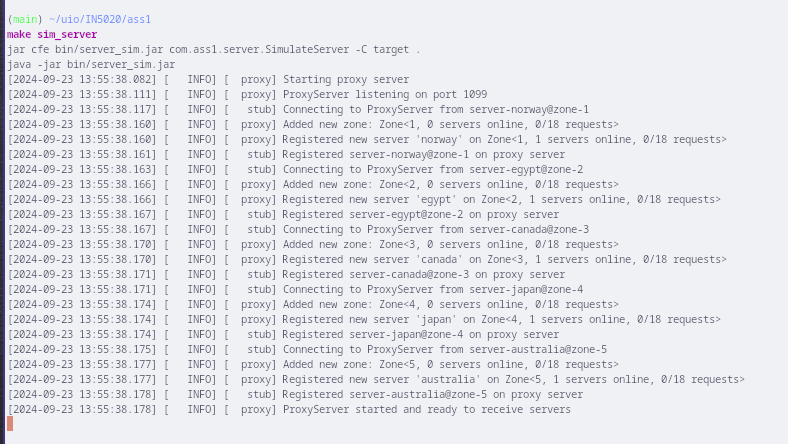
\includegraphics[width=0.9\linewidth]{in5020_oblig1_execution_server.png}
    \caption{Server bootup}
    \label{fig:server-boot}
\end{figure}

\begin{figure}
    \centering
    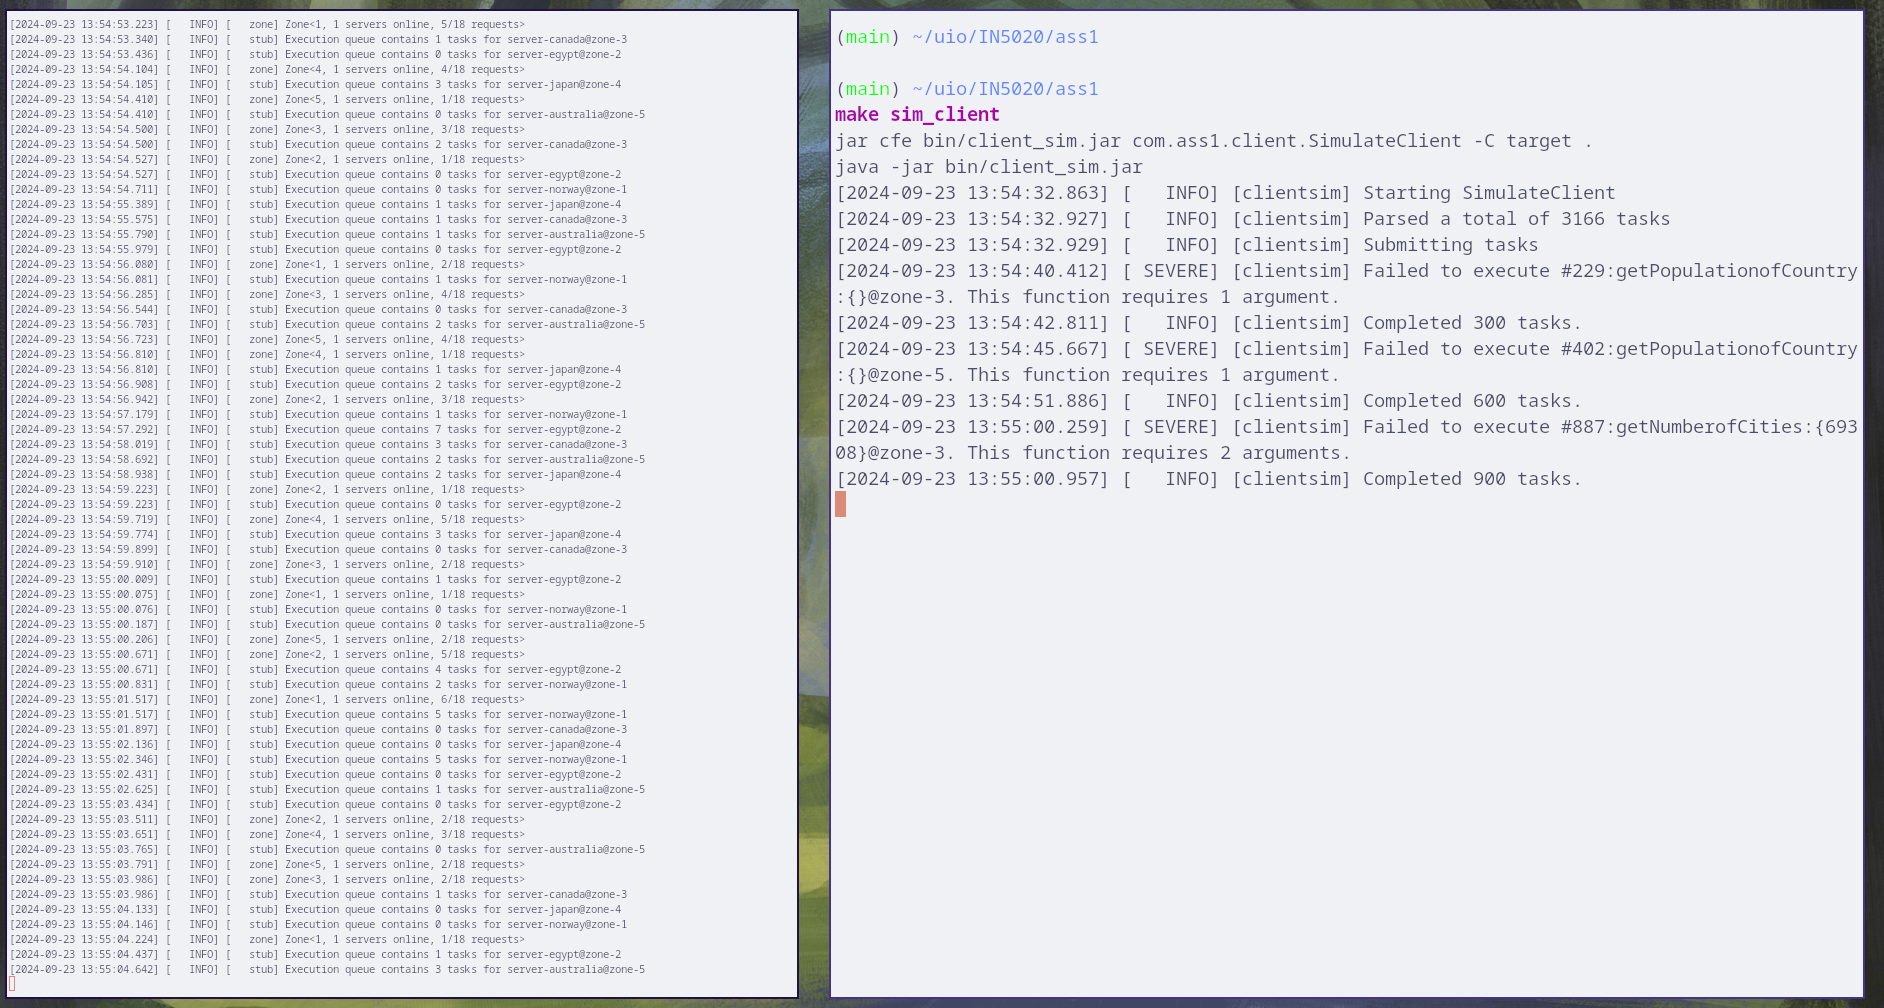
\includegraphics[width=0.9\linewidth]{in5020_oblig1_execution_client.png}
    \caption{Client execution}
    \label{fig:client-execute}
\end{figure}

We run the client simulation for a while, as seen in figure \ref{fig:client-execute}, and can see the execution details being reported on both sides over time. A total of 3166 tasks were given to the server, but we canceled it before completion since it's quite slow.

\subsection{Graphs}
Following we can see the latency over time across the turnaround time (fig. \ref{fig:turnaround-time}), execution time (fig. \ref{fig:execution-time}) and waiting time (fig. \ref{fig:waiting-time}) across all servers.

\begin{itemize}
    \item \textbf{Execution time} refers to the moment the server stub starts computing a query until it knows the answer.
    \item \textbf{Waiting time} refers to the interval from a stub receiving a request until it knows the answer.
    \item \textbf{Turnaround time} refers to the time it takes for a client to send a request until it gets a reply from the server.
\end{itemize}

\begin{figure}
    \centering
    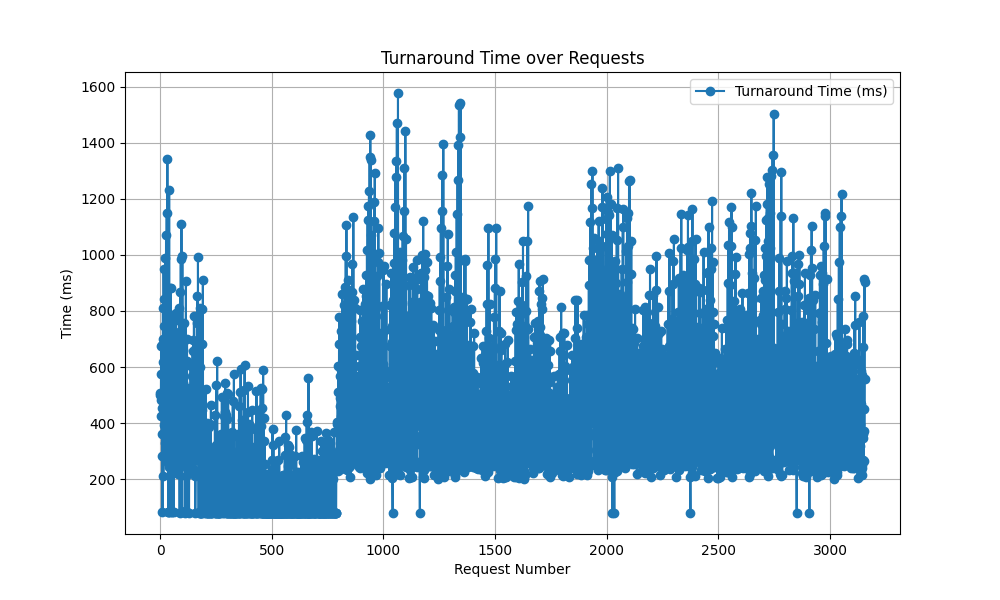
\includegraphics[width=1.0\linewidth]{Turnaround Time.png}
    \caption{Turnaround time, client side}
    \label{fig:turnaround-time}
\end{figure}

\begin{figure}
    \centering
    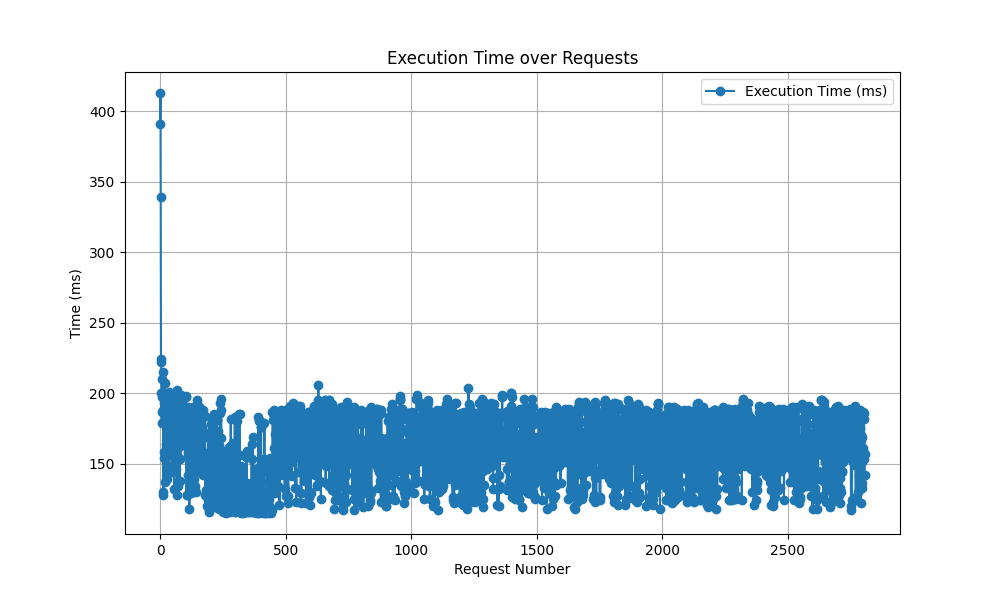
\includegraphics[width=1.0\linewidth]{Execution Time.png}
    \caption{Execution time, server side}
    \label{fig:execution-time}
\end{figure}

\begin{figure}
    \centering
    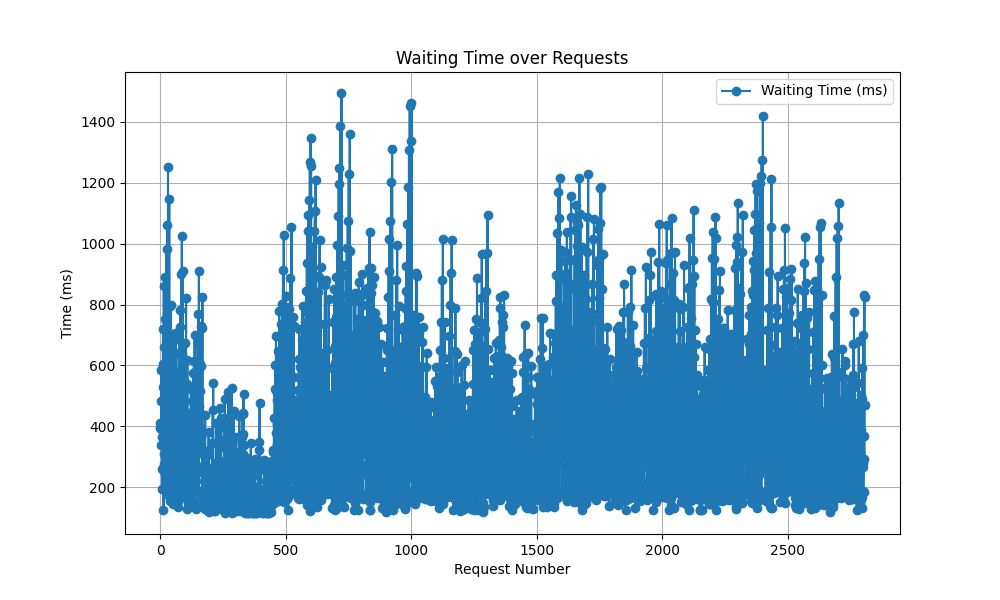
\includegraphics[width=1.0\linewidth]{Waiting Time.png}
    \caption{Waiting time, server side}
    \label{fig:waiting-time}
\end{figure}

\section{Discussion}
\subsection{Result}
\ref{fig:server-boot} and \ref{fig:client-execute} show that we have a working server and client that can connect. The client can send a request through the proxy server and the server will compute and send the result to the corresponding client (simplified). 

All the graphs show the performance of the system. 

\subsection{Error in the pre-code}
Some of the simulated inputs provided by the exercise are malformed. We report these as warnings to the user and skip them.

\section{Workflow}
This project was made as a group effort, using \code{git} to synchronize changes to the codebase between all members.  We all have different system environments, meaning we needed a workflow that was suitable for everyone.

In order to compile the project we, primarily used \code{Makefile}s, minimizing the amount of rebuilding needed to be done on a single change. The abstractions provided by Maven, while useful in certain scenarios, are complete overkill for a project that makes no use of external libraries, and makes certain things unnecessarily complicated, so we decided to gut it.

We decided to use Java 21 for no other reason than that it is the latest LTS version of Java at project start. Specifically, we've used OpenJDK 21, but any modern version version of Java will probably work. For more details on how to compile and run the project, check the \code{README} and \code{Makefile} on the root of the project repository. 

\subsection{Participation}
From the two weeks we had to make this project, we only had one week with a fully established team. Lise and Mazunki started the project before our team was fully formed, and were, therefore, more familiar with the code than Mouaz who joined later. On top of this, due to real-life scheduling (e.g., work and lectures), we haven't had many moments where we could all work together to share ideas over a board.

The specifics of who did what are roughly available on the git repository commit history but are somewhat misleading. It doesn't account for meetings and discussions on how to build the architecture, and which decisions were made on a whiteboard.

There is no clear cut between who was responsible for which part, but Lise mostly worked on the Client and Server implementation, testfiles, and architectural decisions; Mazunki did most of the implementation of the load balancer, client-server interfaces and stubs, and setting up the Makefile and shellscripts; while Mouaz, who came in later, took care of the caching, plotting the time measurement graphs, and fixing the output files required for the delivery.

\section{Conclusion}
In general, we consider that the scope of this assignment is too dense for the time we were given. This may partially be explained by the delay caused between creating a group and actually starting the project, but we estimate that we have worked a combined 120 hours on the assignment, and haven't had time to go over our work to polish off the edge cases. But from the tests and needed graphs we believe that the system works as needed.
\end{document}

